%!TEX root = ../trabajo.tex
	\begin{tabular}{ c  p{11cm} }
    		\raisebox{-\totalheight}{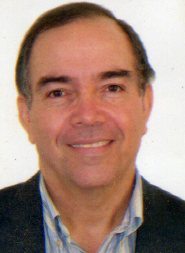
\includegraphics[width=0.15\textwidth]{graficas/CarlosL.jpg}}
    		& 
     	\begin{itemize}[topsep=0.1pt]
     }
     	\item[] 	\begin{Large}
     	\textbf{CARLOS  LAMEDA MONTERO}
     	\end{Large}
     	\item[] \textbf{RESUMEN CURRICULUM VITAE}
     	\end{itemize}	
     \end{tabular}

\begin{footnotesize}

   	\begin{itemize}
   	\item Ingeniero Electrónico, Instituto Universitario Politécnico de Barquisimeto, Venezuela, 1975.
    \item Master of Science en Ingeniería Eléctrica, Universidad de Stanford, USA, 1979.
 	\item Diploma de Estudios Avanzados en el área de Ingeniería de Sistemas y Automática, UNED, España, 2002.
 	\item Maestría en Ciencias de la Computación, Mención Inteligencia Artificial, UCLA, Venezuela, 2003.
	\item Estudios de Doctorado en Ciencias de la Ingeniería Mención Productividad, Universidad Nacional Experimental Politécnica Antonio José de Sucre (UNEXPO), escolaridad concluida en abril de 2015.
	\item Docente de la (UNEXPO), desde 1975 hasta el presente (2015).  Profesor Titular desde 1989.
	\item Jefe de la Sección de Control y Computación, Departamento de Ingeniería Electrónica, UNEXPO, 1980-87 y 1990-94.
	\item Director de Investigación y Postgrado, UNEXPO, Vicerrectorado Barquisimeto, 1995-1999.
Profesor jubilado de la UNEXPO desde marzo 2000.
	\item Coordinador de la Maestría en Ingeniería Electrónica de la UNEXPO (marzo 2003 – marzo 2007).
	\item De enero 2006 a abril 2016, Profesor de postgrado de las asignaturas Computación Emergente Aplicada a las Telecomunicaciones, Seminario de Investigación en Electrónica, Control Digital, Control Inteligente, Laboratorio de Simulación de Control Avanzado de Procesos, Control Adaptativo, Taller de Elaboración de Trabajo de Grado (UNEXPO), Lógica Difusa y Redes Neuronales, Modelos Lineales Aplicados a la Industria de Alimentos (UNELLEZ), Inteligencia Artificial, Sistemas Neurodifusos (Universidad de Carabobo), Sistemas Expertos (UCLA), Instrumentación Electrónica Avanzada (UNET).
   	\end{itemize}     
\newpage

\textbf{OTROS MÉRITOS Y ACTIVIDADES:}
 	\begin{itemize}
 	
 	\item Diseñador de la Opción Computación en Ingeniería Electrónica de la UNEXPO, 1982-1985.	
	\item Autor de 6 libros textos y guías de estudio de ingeniería.
	\item Autor de 36 trabajos de investigación.
	\item Coordinador de la Unidad de Proyectos Especiales (1996-1999), la cual ha recibido los premios  Innovación Tecnológica "Armada 97" (1997) y Excelencia Académica UNEXPO (1999). 
	\item Miembro de la Junta Administradora de la empresa pública ENELBAR (abril 2001- mayo 2003).
	\item Integrante de la Comisión Regional Centroccidental del Sistema para el Reconocimiento de Méritos a los Profesores de las Universidades Nacionales (2003). 
	\item Integrante de Comités Evaluadores de las Maestrías en Ingeniería Electrónica USB (2004) y UNET (2006), designado por el Consejo Nacional de Universidades (CNU). 
	\item “Technical Assistant” del equipo Waroz-UCLA, sub-campeón de la región Norte de Sur América ACM-ICPC World Internacional Programming Contest, participante en la final mundial, Tokio, Japón, abril 2007. 
	\item Conferencista en el VI Congreso Internacional de Electrónica y Tecnologías de Avanzada, Universidad de Pamplona, Colombia, marzo 2008. 
	\item Premios por trabajo de investigación y por trayectoria como investigador UNEXPO (1993), CONABA (1996), Orden "General Juan Jacinto Lara" 1ª Clase (1996), CONADES (1998), PPI (2005), PPI (2008), PEI (2011), PEI (2013), PEI (2015).
	\item Coordinador Iberoamericano de proyecto financiado por la Agencia Española de Cooperación Internacional para el Desarrollo (AECID) en colaboración con la UNED y la UNEXPO (2008-2009).
	\item Miembro de los Comités Organizadores de los Seminarios Nacionales sobre “Borrosidad y Sistemas Difusos”, “Inteligencia Artificial: Un Panorama de Aplicaciones” y “Modelos y Modelado” (2001-2015). 
    \item Conferencista en el I Congreso Internacional de Ingeniería de Sistemas en Inteligencia Computacional, Universidad Simón Bolívar sede Cúcuta, Colombia, septiembre 2015. 	
 	
 	\end{itemize}
\textbf{TRABAJOS DE GRADO DE MAESTRÍA TUTORADOS}

  \begin{flushleft}

\textbf{Año: 2016. Institución: Universidad Nacional Experimental Politécnica “Antonio José de Sucre” (UNEXPO)}\\
\begin{itemize}
\item “Sintonización de Controladores PID en Procesos de Primer y Segundo Orden Mediante Optimización por Enjambre de Partículas”\\
Nombre del estudiante: Henry Zapata\\ 
Título a Obtener: Magíster Scientiarum en Ingeniería de Control de Procesos    
\end{itemize}
  
\textbf{Año: 2014. Institución: Universidad Nacional Experimental Politécnica “Antonio José de Sucre” (UNEXPO)}\\
\begin{itemize}
\item “Control Difuso de la Velocidad Angular para una Turbina Eólica”\\
Nombre del estudiante: Manuel Díaz\\ 
Título a Obtener: Magíster Scientiarum en Ingeniería de Control de Procesos \\
\item “Control Adaptativo de Temperatura para un Reactor Continuo tipo Tanque Agitado”
Nombre del estudiante: Gerson Urbina 
Título a Obtener: Magíster Scientiarum en Ingeniería de Control de Procesos 
\end{itemize}

\textbf{Año: 2013. Institución: Universidad Nacional Experimental Politécnica “Antonio José de Sucre” (UNEXPO)}\\
\begin{itemize}
\item “Control de la Concentración de Etanol en el Tope de una Columna de Destilación Continua mediante un Sistema Adaptativo de Inferencia Neurodifusa”\\
Nombre del estudiante: Eumar Leal\\
Título a Obtener: Magíster Scientiarum en Ingeniería de Control de Procesos
\item “Control Robusto de la Concentración de Etanol en un Proceso de Cultivo Semicontinuo de Levaduras”\\
Nombre del estudiante: Antioquía Galicia\\
Título a Obtener: Magíster Scientiarum en Ingeniería de Control de Procesos 
\end{itemize}

\textbf{Año: 2013. Institución: Universidad Centroccidental Lisandro Alvarado (UCLA)}\\
\begin{itemize}
\item “Modelo Basado en Lógica Difusa para la Comparación de Objetos con Atributos Imprecisos”\\
Nombre del estudiante: Sheijer Silva\\
Título Obtenido: Magíster Scientiarum en Ciencias de la Computación.
\end{itemize}

\textbf{Año: 2011. Institución: Universidad Nacional Experimental Politécnica “Antonio José de Sucre” (UNEXPO)}\\
\begin{itemize}
\item “Software de Soporte para el Proceso de Enseñanza-Aprendizaje de un Laboratorio de Comunicaciones Digitales”\\
Nombre del estudiante: Celeste Leopardi\\
Título a Obtener: Magíster Scientiarum en Ingeniería Electrónica 
\item “Control Predictivo de Nivel de Agua y Presión de Vapor  para una Caldera”\\
Nombre del estudiante: Fermín García\\
Título a Obtener: Magíster Scientiarum en Ingeniería de Control de Procesos 
\end{itemize}


\textbf{Año: 2010. Institución: Universidad Nacional Experimental Politécnica “Antonio José de Sucre” (UNEXPO)}\\
\begin{itemize}
\item “Control Adaptativo de la Concentración de Etanol en un Proceso de Cultivo Semicontinuo de Levaduras”\\
Nombre del estudiante: Luz Marina Suárez\\
Título a Obtener: Magíster Scientiarum en Ingeniería de Control de Procesos
\item “Sistema de Control Difuso para la Alimentación de Sustrato en un Cultivo Semicontinuo de Levaduras”\\
Nombre del estudiante: Llelysmar Crespo\\
Título Obtenido: Magíster Scientiarum en Ingeniería de Control de Procesos 
\end{itemize}

\textbf{Año: 2009. Institución: Universidad Nacional Experimental Politécnica “Antonio José de Sucre” (UNEXPO)}\\
\begin{itemize}
\item “Control Difuso de Temperatura para un Horno a Gas”\\
Nombre del estudiante: Giovanny Rodríguez\\
Título Obtenido: Magíster Scientiarum en Ingeniería de Control de Procesos 
\item “Evaluación del Desempeño de Sistemas Neuro-Difusos en la Identificación de Canales de Radiocomunicaciones”\\ 
Nombre del estudiante: Ángel José León Peña\\
Título Obtenido: Magíster Scientiarum en Ingeniería Electrónica 
\end{itemize}

\textbf{Año: 2009. Institución: Universidad de Carabobo (UC). Título Obtenido: Magíster Scientiarum en Ingeniería Eléctrica}\\
\begin{itemize}

\item “Consultor Inteligente  para el Mantenimiento  de Redes LAN de Alta Velocidad Ethernet Basado en Agentes Inteligentes”\\
Nombre del estudiante: Marisela Materano
\item “Diseño de  un Sistema Experto para el Asesoramiento en las Operaciones de Mantenimiento de Redes WLAN Basado en Árboles de Decisión”\\
Nombre del estudiante: Yelmin Pérez
\end{itemize}
 
\textbf{Año: 2007. Institución: Universidad Centroccidental Lisandro Alvarado (UCLA)}\\
\begin{itemize}
\item “Sistema para la Determinación del Flujo en un Canal Vehicular Basado en Procesamiento de Imágenes y Redes Neuronales”\\  
Nombre del estudiante: Antonio Ferraz\\
Título Obtenido: Magíster Scientiarum en Ciencias de la Computación.
\end{itemize}

\textbf{Año: 2005. Institución: Universidad Centroccidental Lisandro Alvarado (UCLA)}\\
\begin{itemize}
\item “Sistema de Clasificación Neurodifusa en Imágenes de Envases”\\
Nombre del estudiante: Oscar Galindo\\
Título Obtenido: Magíster Scientiarum en Ciencias de la Computación.
\end{itemize}


\textbf{Año: 1997. Institución: Universidad Nacional Experimental Politécnica “Antonio José de Sucre” (UNEXPO)}\\
\begin{itemize}
\item “Diseño de un Controlador Digital Utilizando el Puerto Paralelo de un PC”\\
Nombre del estudiante: Carlos  Alberto Rey Soto\\
Título Obtenido: Magíster Scientiarum en Ingeniería Electrónica  
\end{itemize}

\textbf{Año: 1996.  Institución: UNEXPO}\\ 
\begin{itemize}
\item “Diseño y Construcción de un Electrocardiógrafo de un Canal Basado en Microcontroladores, Capaz de Funcionar como Sistema Remoto de Adquisición de Señal Eléctrica Cardíaca para un PC”\\ 
Nombre del estudiante: Humberto Barazarte\\
Título Obtenido: Magíster Scientiarum en Ingeniería Electrónica 
\item “Aplicación de Controladores Lógicos Programables “PLC”  en un Proceso Industrial de Trituración y Homogenización”\\ 
Nombre del estudiante: José Heliodoro Quintero\\
Título Obtenido: Magíster Scientiarum en Ingeniería Electrónica 
\item “Diseño e Implementación de un Sistema de Monitoreo por Computador de la Variables: Nivel, Temperatura y Flujo para una planta de Procesos Piloto”\\
Nombre del estudiante: Virgilio Baptista\\
Título Obtenido: Magíster Scientiarum en Ingeniería Electrónica 
\end{itemize}
 \end{flushleft}
\textbf{  ALGUNAS PUBLICACIONES}
\begin{flushleft}
\begin{itemize}
\item “ANFIS Neuro-Fuzzy modeling of a pneumatic leak testing system”. CDC-ECC 05, Sevilla, España. Diciembre 2005.
\item “La Inteligencia artificial y sus aportes a la física médica y la bioingeniería. En Publicaciones de la Comisión de Estudios Interdisciplinarios, UCV, Año 9, No 24, 2006, pp. 149-153.
\item “Clasificación de Lesiones Gástricas en Imágenes Endoscópicas mediante la Técnica de Pirámide Difusa  y Redes Neuronales”. CLAIB 2007. Venezuela, septiembre 2007.
\item “Herramienta computacional para la combinación balanceada de nutrientes utilizando lógica difusa y búsqueda heurística”, Revista de Ciencia y Tecnología Agrollanía, Volumen 5, 2008, pp. 1-10.
\item “Clasificador difuso neuronal aplicado a casos de enfermedades hepatobiliares representadas por datos con patrones solapados”,  Revista  Científica UNET, Volumen 20 Nº,1 2008, pp. 85-98.
\item “Extracción automática de características de vehículos en movimiento a partir de videos basada en red neuronal de Kohonen”.  Revista   Ingeniería UC, Volumen 15, N° 3, 2008, pp. 33-44.
\item “Design of a pH and temperature fuzzy control system for the production process of liquid ammonium nitrate”. 3rd Seminar for Advanced Industrial Control Applications. SAICA 2009. Madrid, España. 
\item “Sistema de control difuso para la alimentación de sustrato en un cultivo semicontinuo de levaduras”. XIV Congreso Latinoamericano de Control Automático, Santiago de Chile, agosto 2010.
\item “El Análisis Envolvente de Datos y el Índice de Malmquist como Técnicas Innovadoras en el Análisis de la Eficiencia y Productividad en Departamentos Académicos de Universidades Venezolanas”. Congreso Regional de Investigación y Pedagogía 2014. UPEL, Barquisimeto, Venezuela.
\item “Control para Alimentación de Sustrato en Cultivo De Lactococcus lactis”. 24º Congreso Argentino de Control Automático, 27 al 29 de Octubre de 2014 – Buenos Aires, Argentina.
\item “Métodos Relacionados con Diagnósticos de Fallas con Síntomas Imprecisos mediante Comparación ce Casos”. REDIP. Venezuela. Vol. 5. No. 3, 2015.
\item “Importancia de Publicar Artículos Científicos desde las Perspectivas Individual, de las Organizaciones y La Sociedad”. REDIP. Venezuela. Vol. 5. No. 4, 2015.

\end{itemize}
\end{flushleft}
\end{footnotesize}